\documentclass{article}

\usepackage{arxiv}

\usepackage[utf8]{inputenc} % allow utf-8 input
\usepackage[T1]{fontenc}    % use 8-bit T1 fonts
\usepackage{hyperref}       % hyperlinks
\usepackage{url}            % simple URL typesetting
\usepackage{booktabs}       % professional-quality tables
\usepackage{amsfonts}       % blackboard math symbols
\usepackage{nicefrac}       % compact symbols for 1/2, etc.
\usepackage{microtype}      % microtypography
\usepackage{lipsum}
\usepackage{graphicx}

\usepackage{listings}
\usepackage{xcolor}

\definecolor{codegreen}{rgb}{0,0.6,0}
\definecolor{codegray}{rgb}{0.5,0.5,0.5}
\definecolor{codepurple}{rgb}{0.58,0,0.82}
\definecolor{backcolour}{rgb}{0.95,0.95,0.92}

\lstdefinestyle{mystyle}{
    backgroundcolor=\color{backcolour},   
    commentstyle=\color{codegreen},
    keywordstyle=\color{magenta},
    numberstyle=\tiny\color{codegray},
    stringstyle=\color{codepurple},
    basicstyle=\ttfamily\footnotesize,
    breakatwhitespace=false,         
    breaklines=true,                 
    captionpos=b,                    
    keepspaces=true,                 
    numbers=left,                    
    numbersep=5pt,                  
    showspaces=false,                
    showstringspaces=false,
    showtabs=false,                  
    tabsize=2
}

\lstset{style=mystyle}

\graphicspath{ {./img/} }

\title{mate-ai-one: a simple chess engine}

\author{
 Matteo Galiazzo \\
  Dipartimento di Informatica - Scienza e Ingegneria\\
  Università di Bologna\\
  \texttt{matteo.galiazzo@studio.unibo.it} \\
  %% examples of more authors
   \And
 Nicola Modugno\\
  Dipartimento di Informatica - Scienza e Ingegneria\\
  Università di Bologna\\
  \texttt{mail@studio.unibo.it} \\
  \And
 Daniele Russo\\
  Dipartimento di Informatica - Scienza e Ingegneria\\
  Università di Bologna\\
  \texttt{mail@studio.unibo.it} \\
  %% \AND
  %% Coauthor \\
  %% Affiliation \\
  %% Address \\
  %% \texttt{email} \\
  %% \And
  %% Coauthor \\
  %% Affiliation \\
  %% Address \\
  %% \texttt{email} \\
  %% \And
  %% Coauthor \\
  %% Affiliation \\
  %% Address \\
  %% \texttt{email} \\
}

\begin{document}
\maketitle
\begin{abstract}
TODO
\end{abstract}

% keywords can be removed
%\keywords{First keyword \and Second keyword \and More}

\section{Introduction}
Il gioco degli scacchi è sempre stato un banco di prova per strategia, logica e intelligenza, rappresentando una sfida affascinante sia per gli esseri umani che per le macchine.
In questo progetto del corso di Intelligenza Artificiale, ci siamo dedicati allo sviluppo di un bot in grado di giocare a scacchi, arricchito da una barra di valutazione della posizione.
Questo strumento non solo migliora l'interazione con l'utente, ma offre anche una prospettiva dinamica sull'andamento della partita.
Il report che segue illustra il percorso di realizzazione del progetto, evidenziando le scelte progettuali e gli obiettivi raggiunti.

\section{Valutazione della posizione tramite ricerca}

\subsection{Valutazione della posizione}

Vogliamo creare una funzione di valutazione per valutare quanto è buona una posizione.
Per farlo, utilizziamo il semplice metodo di guardare quanti pezzi ha ciascun giocatore e di assegnare a ciascun pezzo un valore.
Il calcolo del valore dei pezzi fornisce ai giocatori solo un'idea del valore statico del materiale, cioè della loro forza intrinseca al di fuori del gioco, posseduto da ambedue i giocatori in un determinato momento del gioco.
L'esatto valore dei pezzi e dei pedoni dipende dalla potenzialità dinamica, cioè dalle loro capacità di movimento e azione nel cuore dello scontro, raggiunta in un preciso momento della partita \cite{wikipediaChessPiece}.
Ci affidiamo per ora a una valutazione semplificata, con i seguenti valori:

\begin{lstlisting}[language=python]
PIECE_VALUES = {
  chess.PAWN: 1,
  chess.KNIGHT: 3,
  chess.BISHOP: 3,
  chess.ROOK: 5,
  chess.QUEEN: 9,
  chess.KING: 0
}
\end{lstlisting}

Per ottenere la valutazione della posizione moltiplichiamo il numero di pezzi di un certo colore per il valore del pezzo, e poi facciamo la differenza tra le due somme.
Notiamo che il valore del re è infinito, perchè la sua perdita causa la perdita della partita \cite{wikipediaChessPiece}.
Modelliamo questo comportamento nella funzione di ricerca, che se non trova mosse disponibili controlla se il re è sotto scacco per capire se la partita è terminata con uno scacco matto oppure con uno stallo.

\begin{lstlisting}[language=python]
def search(depth):
  if depth == 0: return basic_eval()
  moves = list(board.generate_legal_moves())

  if len(moves) == 0:
    if board.is_check():
      return -INF
    return 0
    
  best_evaluation = -INF
  for move in moves:
    board.push(move)
    eval = -search(depth - 1)
    best_evaluation = max(eval, best_evaluation)
    board.pop()

  return best_evaluation
\end{lstlisting}

\subsection{MiniMax with Alpha-Beta pruning}

L'algoritmo di ricerca minimax è semplice ed elegante, e con abbastanza capacità computazionale riesce sempre a trovare la miglior mossa da giocare.
Con gli scacchi però in media ci sono \~30 mosse che un giocatore può fare in qualsiasi stato del gioco.
Questo significa che ogni singolo nodo nell'albero avrà approssimativamente 30 figli diversi.
Denotiamo l'ampiezza dell'albero con $w$.
Ci vogliono \~85 mosse consecutive per finire una partita di scacchi.
Questo significa che l'albero avrà una profondità media di 85.
Denotiamo la profondità dell'albero con $d$.

Possiamo quindi definire $w^d$ che ci mostrerà quante posizioni diverse dobbiamo valutare in media.
Per gli scacchi il numero è quindi $30^{85} \approx 3.592 * 10^{125}$.
Questo ci impedisce quindi di esplorare tutte le mosse possibili.

Ricordiamo però che MiniMax è basato sul fatto che un giocatore cerca di massimizzare la funzione di valutazione mentre l'altro cerca di minimizzarla.
Questo comportamento si riflette direttamente nell'albero di ricerca.
Infatti durante l'attraversamento dalle foglie alla radice abbiamo sempre scelto la miglior mossa possibile per un giocatore, quindi per il bianco abbiamo scelto sempre il valore massimo, e per il nero sempre il valore minimo.

\begin{figure}[htbp]
  \centering
  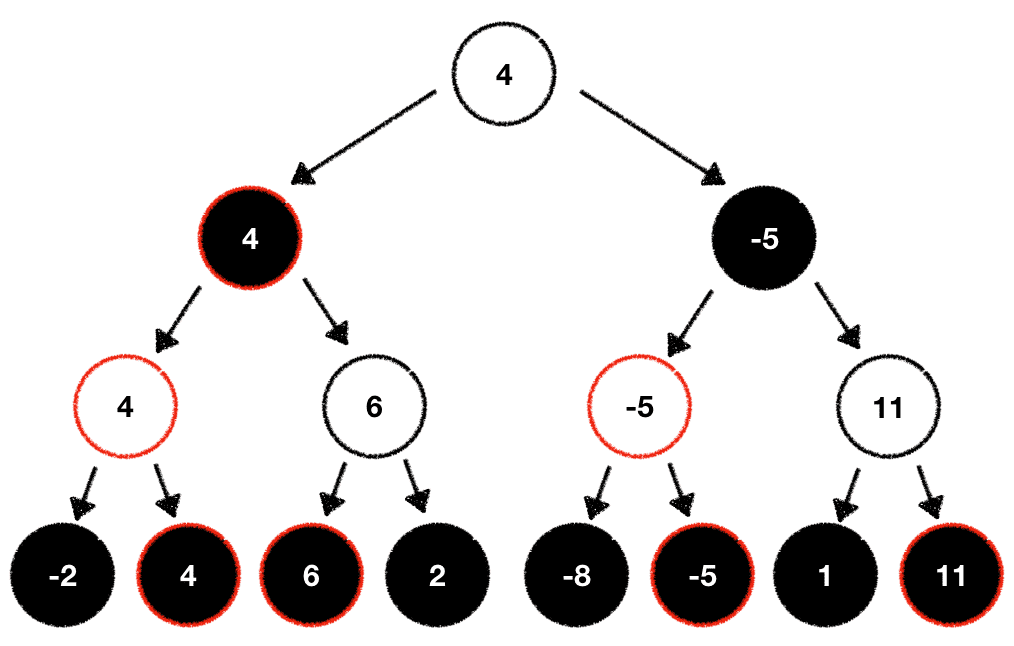
\includegraphics[width=0.75\linewidth]{img/minimax.png}
  \caption{simplified game search tree with selected nodes highlighted}
  \label{fig:minimax}
\end{figure}

Se osserviamo l'albero di ricerca della figura \ref{fig:minimax} possiamo sfruttare questo comportamento per ottimizzarlo.
Mentre facciamo il cammino verso le foglie dovremmo costruire il nostro albero andando prima in profondità (depth-first).
Questo vuol dire che dovremmo iniziare a un nodo ed espanderlo giocando la partita fino alla fine (fino alla profondità di ricerca desiderata) prima di tornare indietro e scegliere il nodo successivo che vogliamo esplorare.
Seguire questa procedura ci permette di identificare prima le mosse che non verranno giocate.
Infatti, un giocatore massimizza il numero (il risultato finale) mentre l'altro lo minimizza.
La parte dell albero di ricerca dove un giocatore finirebbe in una situazione peggiore in base alla funzione di valutazione può essere completamente rimossa dalla lista dei nodi che vogliamo espandere ed esplorare.
Facciamo una potatura (pruning) di questi nodi e quindi riduciamo la larghezza dell'albero.

\begin{figure}[htbp]
  \centering
  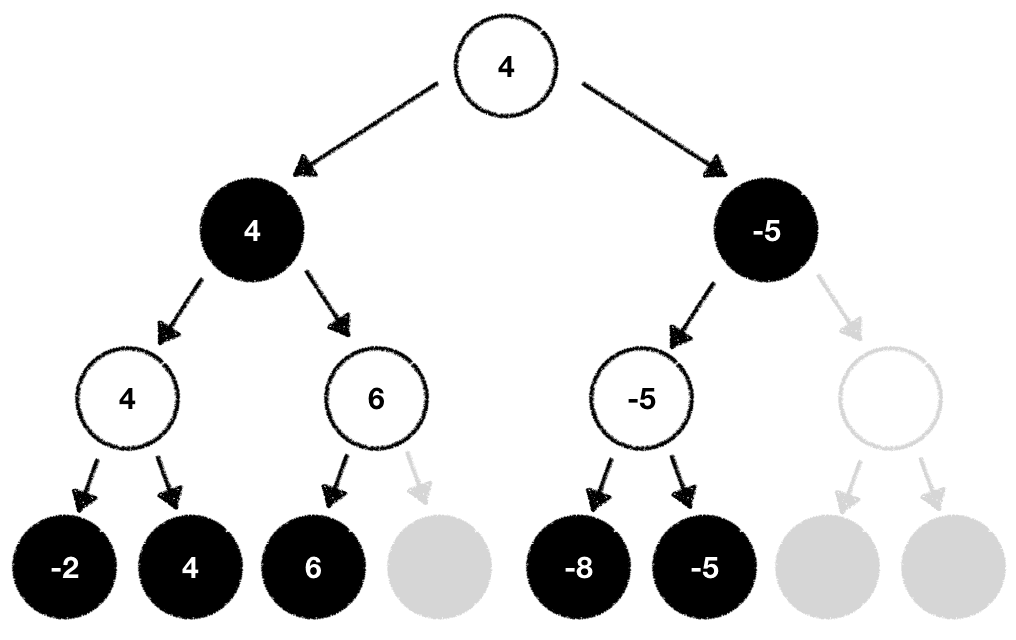
\includegraphics[width=0.75\linewidth]{img/minimax_ab.png}
  \caption{game search tree with pruned nodes}
  \label{fig:minimax_ab}
\end{figure}

Più alto è il branching factor dell'albero, più alto è il numero di calcoli che possiamo risparmiare.

Assumendo di poter ridurre la larghezza di una media di 10 nodi finiremmo con $w^d = (30-10)^{85} \approx 3.868 * 10^{110}$.

Questa tecnica di potatura di parti dell'albero di ricerca è chiamata Alpha-Beta pruning.
Il nome viene dai parametri alpha e beta che vengono utilizzati per tenere traccia del miglior punteggio che ciascun giocatore può ottenere esplorando l'albero.

Il codice per l'Alpha-Beta pruning è:

\begin{lstlisting}[language=python]
eval = search_alphabeta(3, -INF, INF)

def search_alphabeta(depth, alpha, beta):
  if depth == 0: return basic_eval()
  moves = list(board.generate_legal_moves())

  if len(moves) == 0:
    if board.is_check(): return -INF
    return 0
    
  for move in moves:
    board.push(move)
    eval = -search_alphabeta(depth - 1, -beta, -alpha)
    board.pop()
    if eval >= beta: return beta
    alpha = max(alpha, eval)

  return alpha
\end{lstlisting}

Questo ci permette di ridurre drasticamente le posizioni che l'algoritmo deve esplorare nell albero di ricerca.
Nel caso però dell'utilizzo della funzione di valutazione per scegliere la prossima mossa da effettuare, l'algoritmo si perderebbe una cattura nella prossima mossa.
Questo perchè quando l'algoritmo raggiunge la massima profondità di ricerca conteggia il numero di pezzi di ciascun giocatore per capire chi dei due è in vantaggio, ma non ha informazione sulla mossa immediatamente successiva.
L'idea è quindi di iniziare un'altra ricerca alla profondità massima, che considera tutte le catture di pezzi possibili e si ferma solo quando non ci sono più catture disponibili.

\bibliographystyle{unsrt}
\bibliography{references.bib}

\end{document}
